\section{Result and Analysis}
\subsection{Parameters}
\begin{table}[h]
    \centering
    \renewcommand{\arraystretch}{1.5} %
    \begin{tabular}{|c|c|}
        \hline
        \textbf{Parameters}                     & \textbf{Value}      \\
        \hline
        \textbf{Total Datasets}                 & 6                   \\
        \hline
        \textbf{Total images}                   & 446K                \\
        \hline
        \textbf{Trained images (real and fake)} & 203K , 203K         \\
        \hline
        \textbf{Tested images (real and fake)}  & 10K , 10K           \\
        \hline
        \textbf{Validation (real and fake)}     & 10K , 10K           \\
        \hline
        \textbf{Balanced}                       & True                \\
        \hline
        \textbf{Epochs}                         & 10                  \\
        \hline
        \textbf{Batch Size}                     & 32                  \\
        \hline
        \textbf{Image Size}                     & 256 x 256           \\
        \hline
        \textbf{Channels}                       & 3                   \\
        \hline
        \textbf{Patches}                        & 16 x 16             \\
        \hline
        \textbf{Encoder Hidden Layers}          & 12                  \\
        \hline
        \textbf{Encoder Layers Dimension}       & 768                 \\
        \hline
        \textbf{MLP size}                       & 3072                \\
        \hline
        \textbf{ Number of Attention Heads }    & 12                  \\
        \hline
        \textbf{Loss Function}                  & Cross-Entropy Loss  \\
        \hline
        \textbf{Normalization}                  & Layer Normalization \\
        \hline
        \textbf{Activation Function}            & GeLU                \\
        \hline
        \textbf{Dropout Rate }                  & 0.2                 \\
        \hline
        \textbf{Pooling Strategy }              & CLS Token           \\
        \hline
    \end{tabular}
    \caption{Model Parameters}
    \label{tab:model-parameters}
\end{table}
\newpage
\subsection{Evaluation}
\subsubsection{Loss Curve}
\begin{figure}[ht]
    \centering
    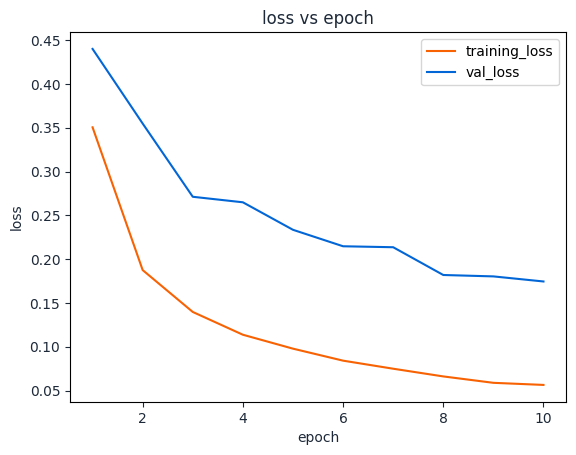
\includegraphics[width= 5in, height =5in ]{img/lossVsAccuracy.png}
    \caption{\textit{Training Vs Validation loss Curve}}
\end{figure}
This plot shows how well our model is doing over time. The horizontal line represents the number of times we've trained the model, and the vertical line shows how well it's performing (lower is better). We have two lines on the graph: one for how well the model is doing during training, and another for how well it's doing on new, unseen data. The goal is to have both lines go down, meaning the model is learning well. By analyzing the "Loss vs. Epoch" plot, one can identify various aspects of the model's performance, such as overfitting, underfitting, and the effectiveness of early stopping.

\newpage
\subsubsection{Accuracy Curve}
\begin{figure}[ht]
    \centering
    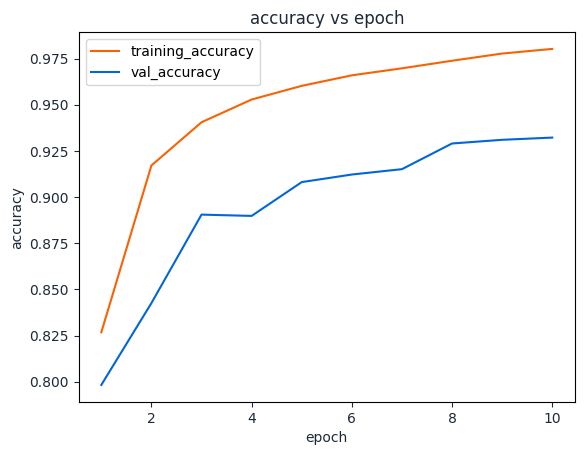
\includegraphics[width=5in, height =5in ]{img/accuracyVsepoch.png}
    \caption{\textit{Training Vs Validation Accuracy Curve }}
\end{figure}
In this graph, the horizontal axis shows the number of training epochs, while the vertical axis represents the accuracy (both training and validation) of our model. Higher accuracy values indicate better overall performance. The plot typically displays two lines: one for training accuracy, reflecting the model's improvement during training, and another for validation accuracy, indicating how well the model generalizes to new, unseen data. Analyzing the "Accuracy vs. Epoch" plot helps identify aspects of the model's performance, including potential overfitting, underfitting, and the effectiveness of early stopping strategies.
With the increase of epoch for validation, unlike loss, there is increase in accuracy.
\newpage
\subsubsection{Confusion Matrix}
\begin{figure}[ht]
    \centering
    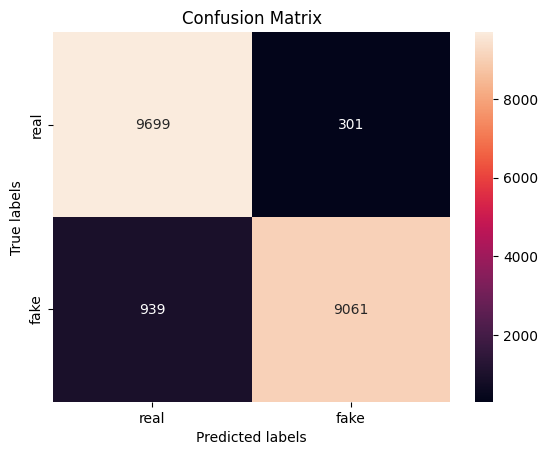
\includegraphics[width=5in, height =5in ]{img/confusionMatrixImage.png}
    \caption{\textit{Confusion Matrix }}
\end{figure}
The confusion matrix is a valuable tool for evaluating our model's ability to classify images as either "real" or "fake." Simply put, it organizes results into a grid where rows represent the actual labels of images, columns depict the predicted labels, and the numbers within cells show how many images fall into each category. For instance, the top-left cell indicates that 9,699 images were correctly identified as real. The diagonal of the matrix reveals that a total of 10,000 images were accurately classified, demonstrating the model's effectiveness. However, the presence of off-diagonal elements, like the bottom-right cell showing 9,061 misclassified fake images, points to areas for improvement. While the model performs well overall, these misclassifications suggest some challenges. Through the confusion matrix, we can dive into more specific metrics like accuracy, precision, recall, and F1-score, offering detailed insights to refine the model's image classification capabilities.
\subsubsection{Performance Metrices}

The performance of our model is associated with various metrics such as:
\begin{enumerate}
    \item \textbf{Accuracy:}
          The accuracy metric measures how correctly the model predicts instances by calculating the ratio of correctly classified instances to the total samples.
          \[ Accuracy = \frac{TP + TN}{TP + FP + TN + FN} \]

    \item \textbf{Precision:}
          Precision assesses the model's ability to identify positive samples among the actual positives, calculated as the ratio of true positives to the sum of true positives and false positives.

          \[ Precision = \frac{TP}{TP + FP} \]

    \item \textbf{Recall (Sensitivity or True Positive Rate):}
          Recall measures the model's ability to precisely identify positive samples from the actual positives, calculated as the ratio of true positives to the sum of true positives and false negatives.

          \[ Recall = \frac{TP}{TP + FN} \]


    \item \textbf{F1 Score:}

          The F1 score, a balance between precision and recall, is advantageous in scenarios with unequal class distribution or equal emphasis on both types of errors. It ranges between 0 and 1, with peak performance at 1.

          \[ F1 = \frac{2 \cdot Precision \cdot Recall}{Precision + Recall} \]

\end{enumerate}
\newpage
\subsection{Model Inference Results }
\begin{enumerate}
    \item \textbf{True Positive:}
         
          \begin{figure}[ht]
              \centering
              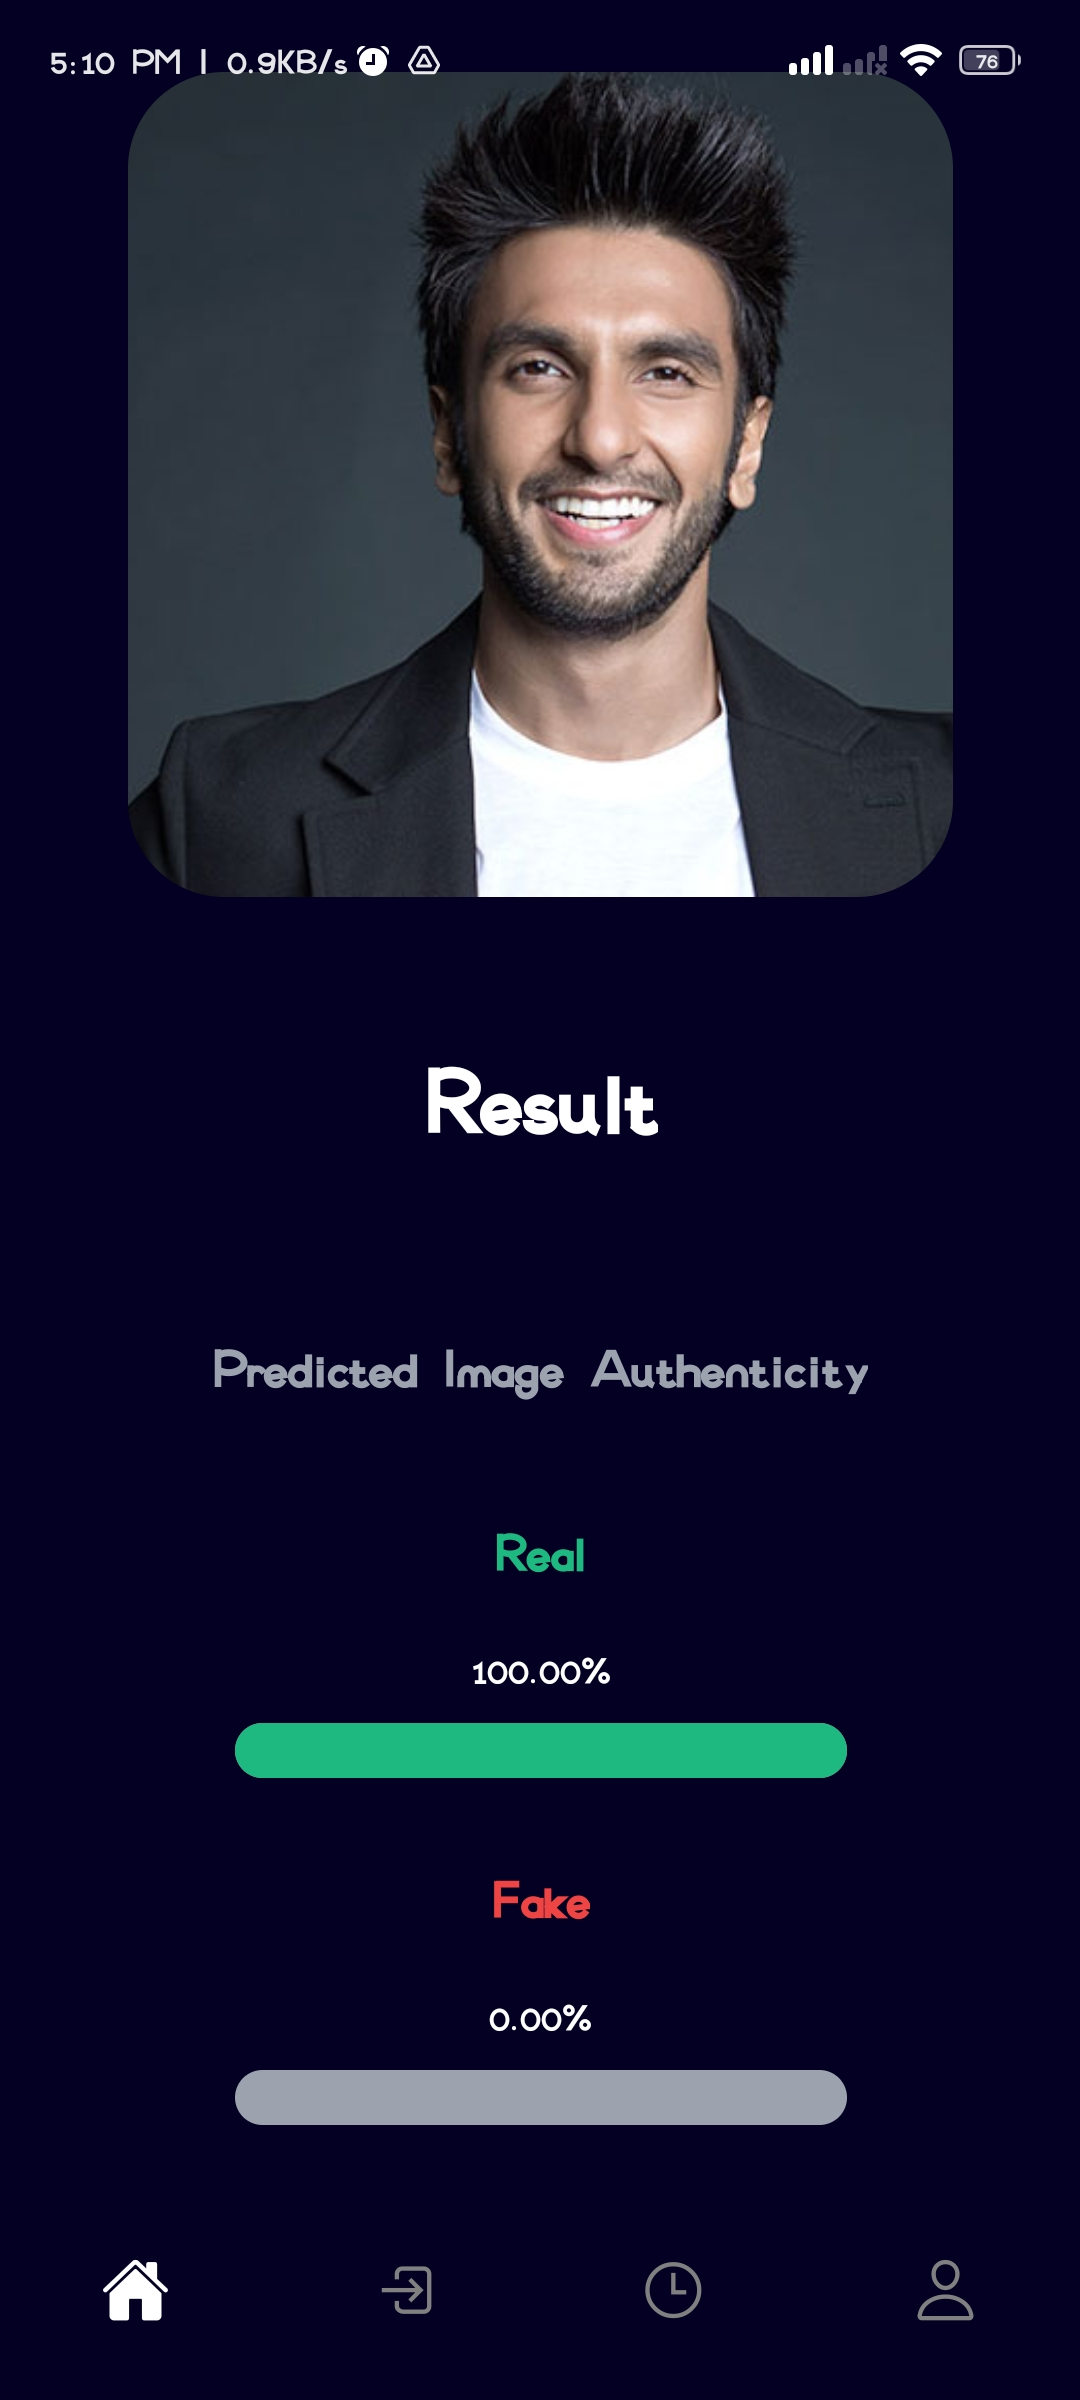
\includegraphics[height =5in  ]{img/ranveerResult.jpg}
              \caption{\textit{Training Vs Validation loss Curve}}
          \end{figure}

          \newpage
    \item \textbf{False Positive:}
       
          \begin{figure}[ht]
              \centering
              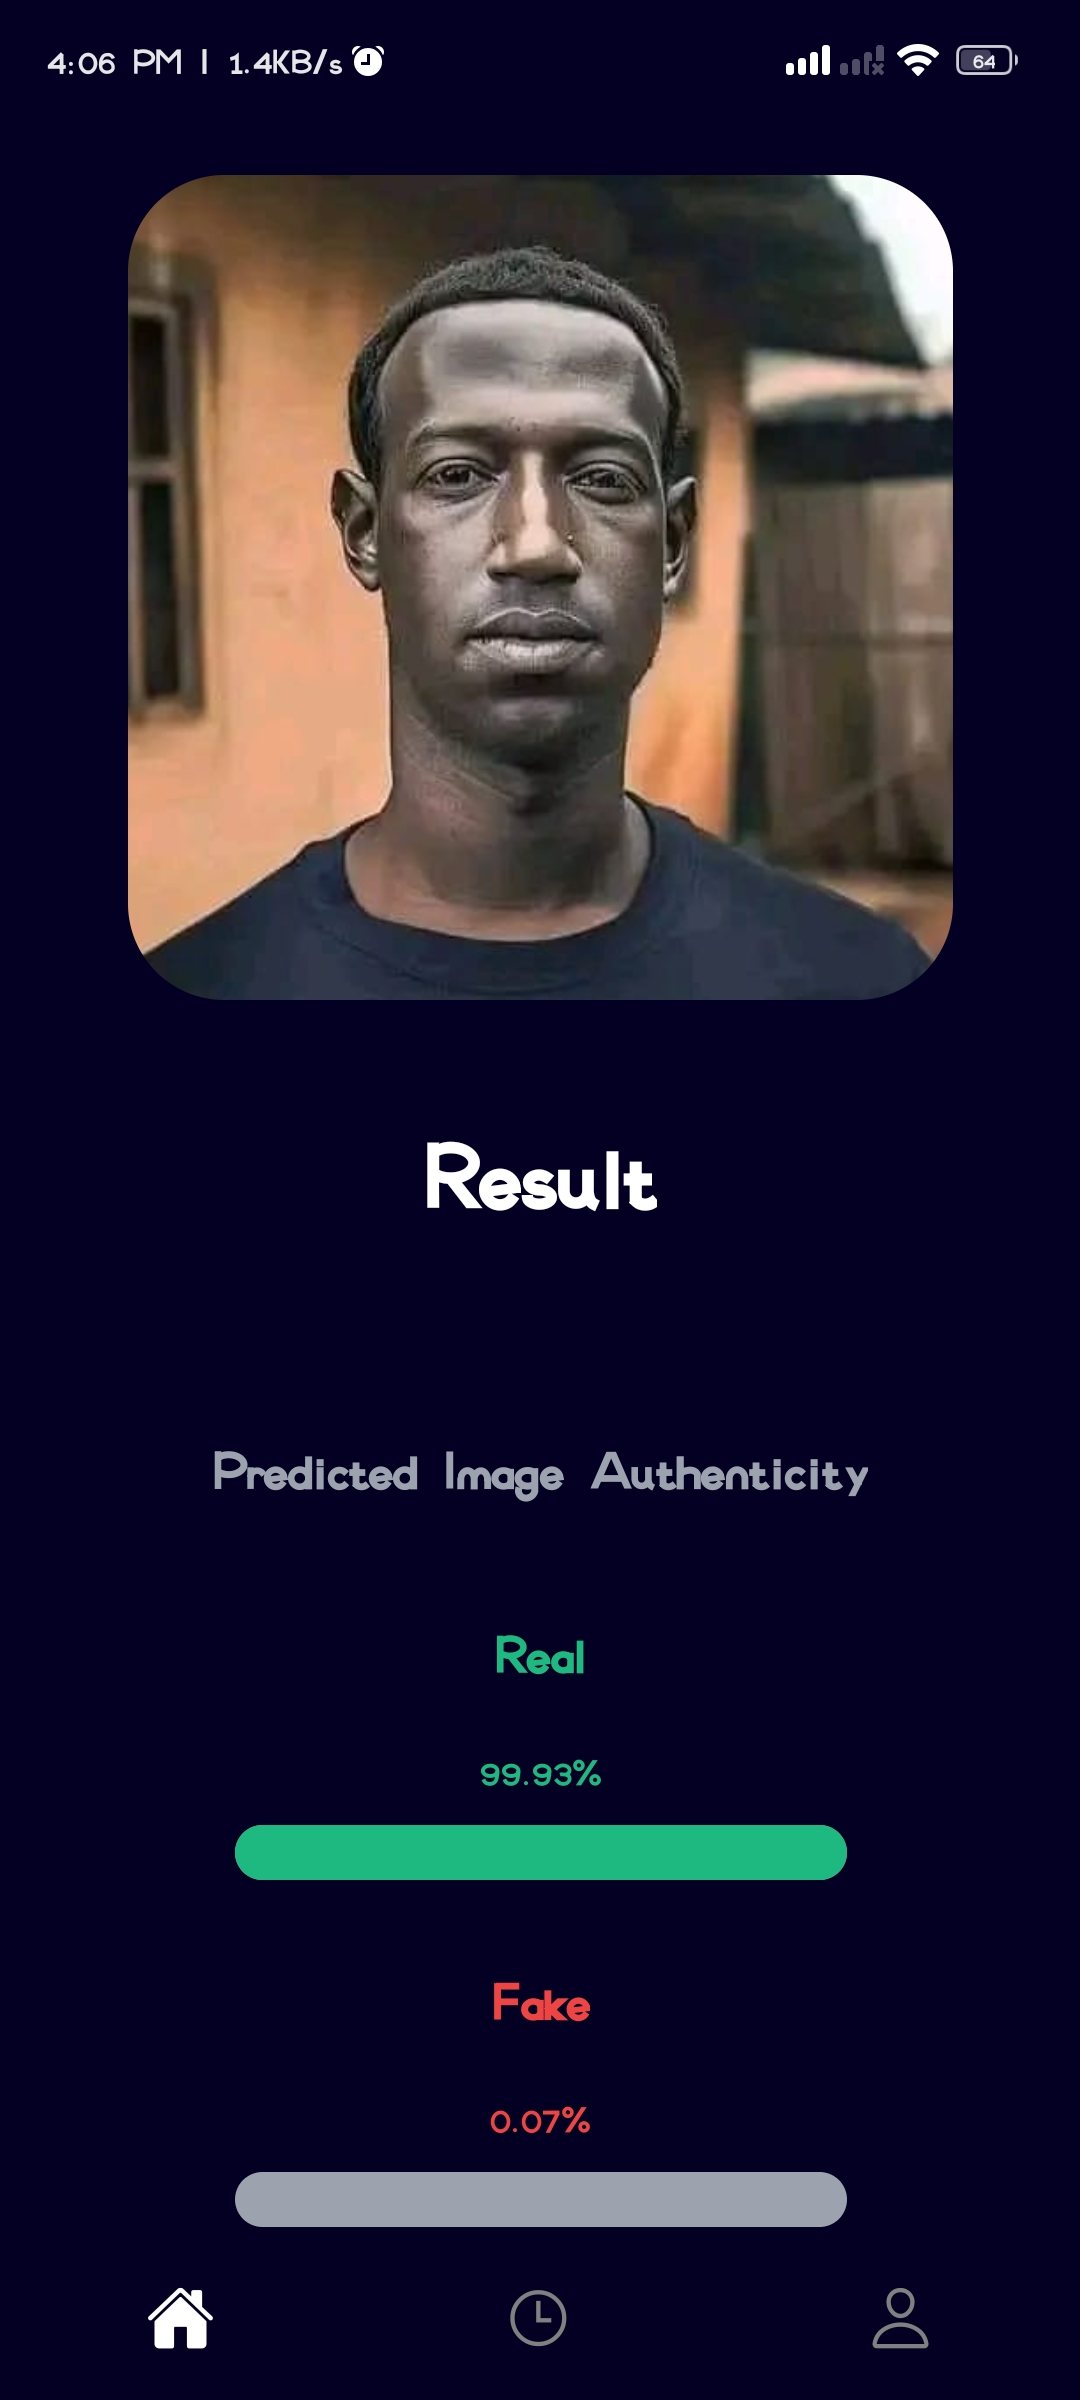
\includegraphics[height =5in  ]{img/blckzukeOutput.jpg}
              \caption{\textit{Training Vs Validation loss Curve}}
          \end{figure}

          \newpage

    \item \textbf{Ture Negative}
      
          \begin{figure}[ht]
              \centering
              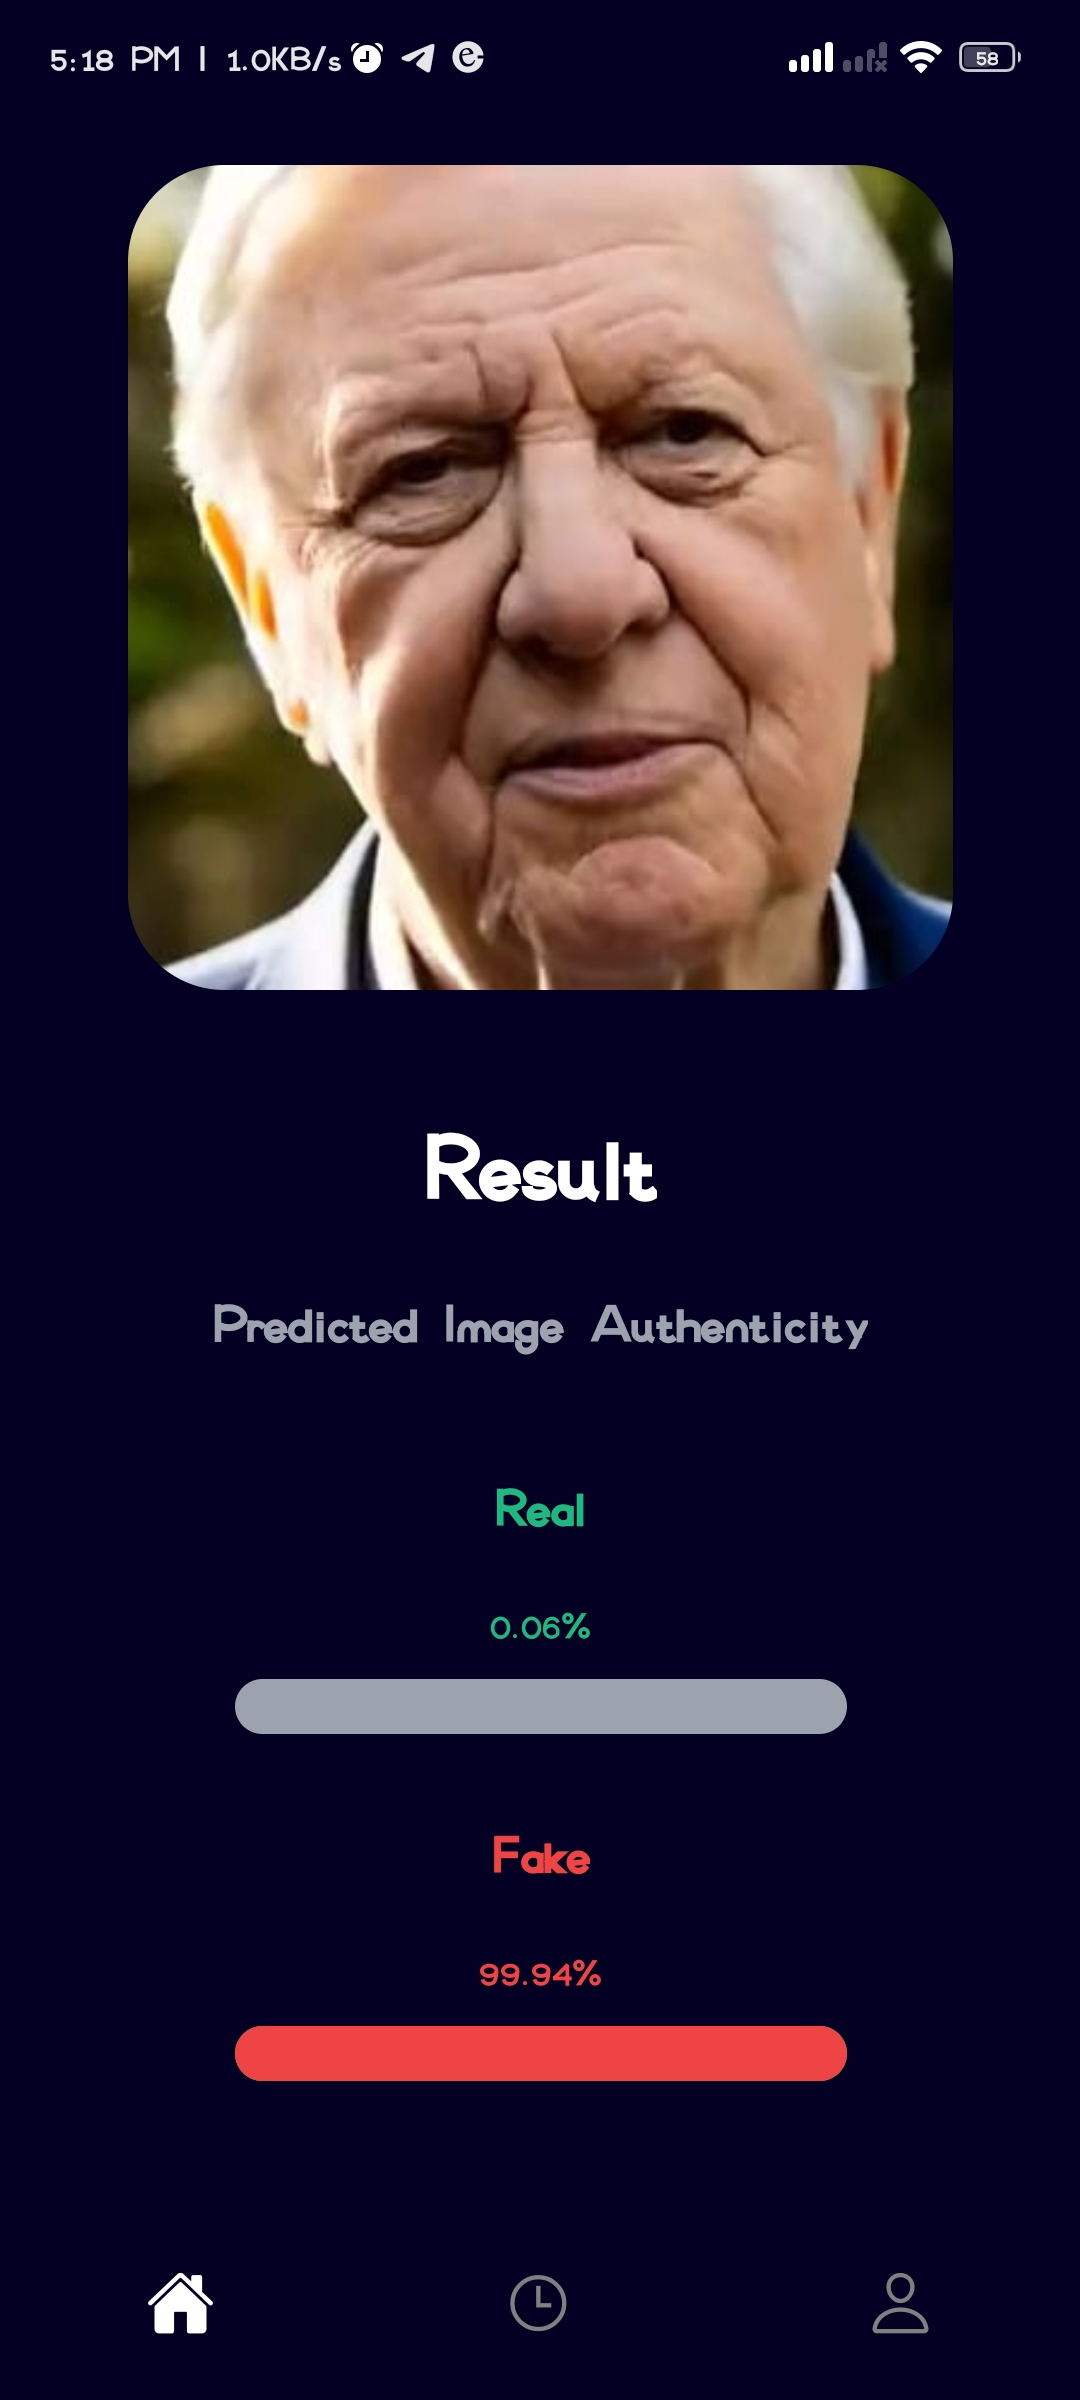
\includegraphics[height =5in ]{img/oldmanResult.jpg}
              \caption{\textit{Training Vs Validation loss Curve}}
          \end{figure}

          \newpage


    \item \textbf{False Negative}
       
          \begin{figure}[ht]
              \centering
              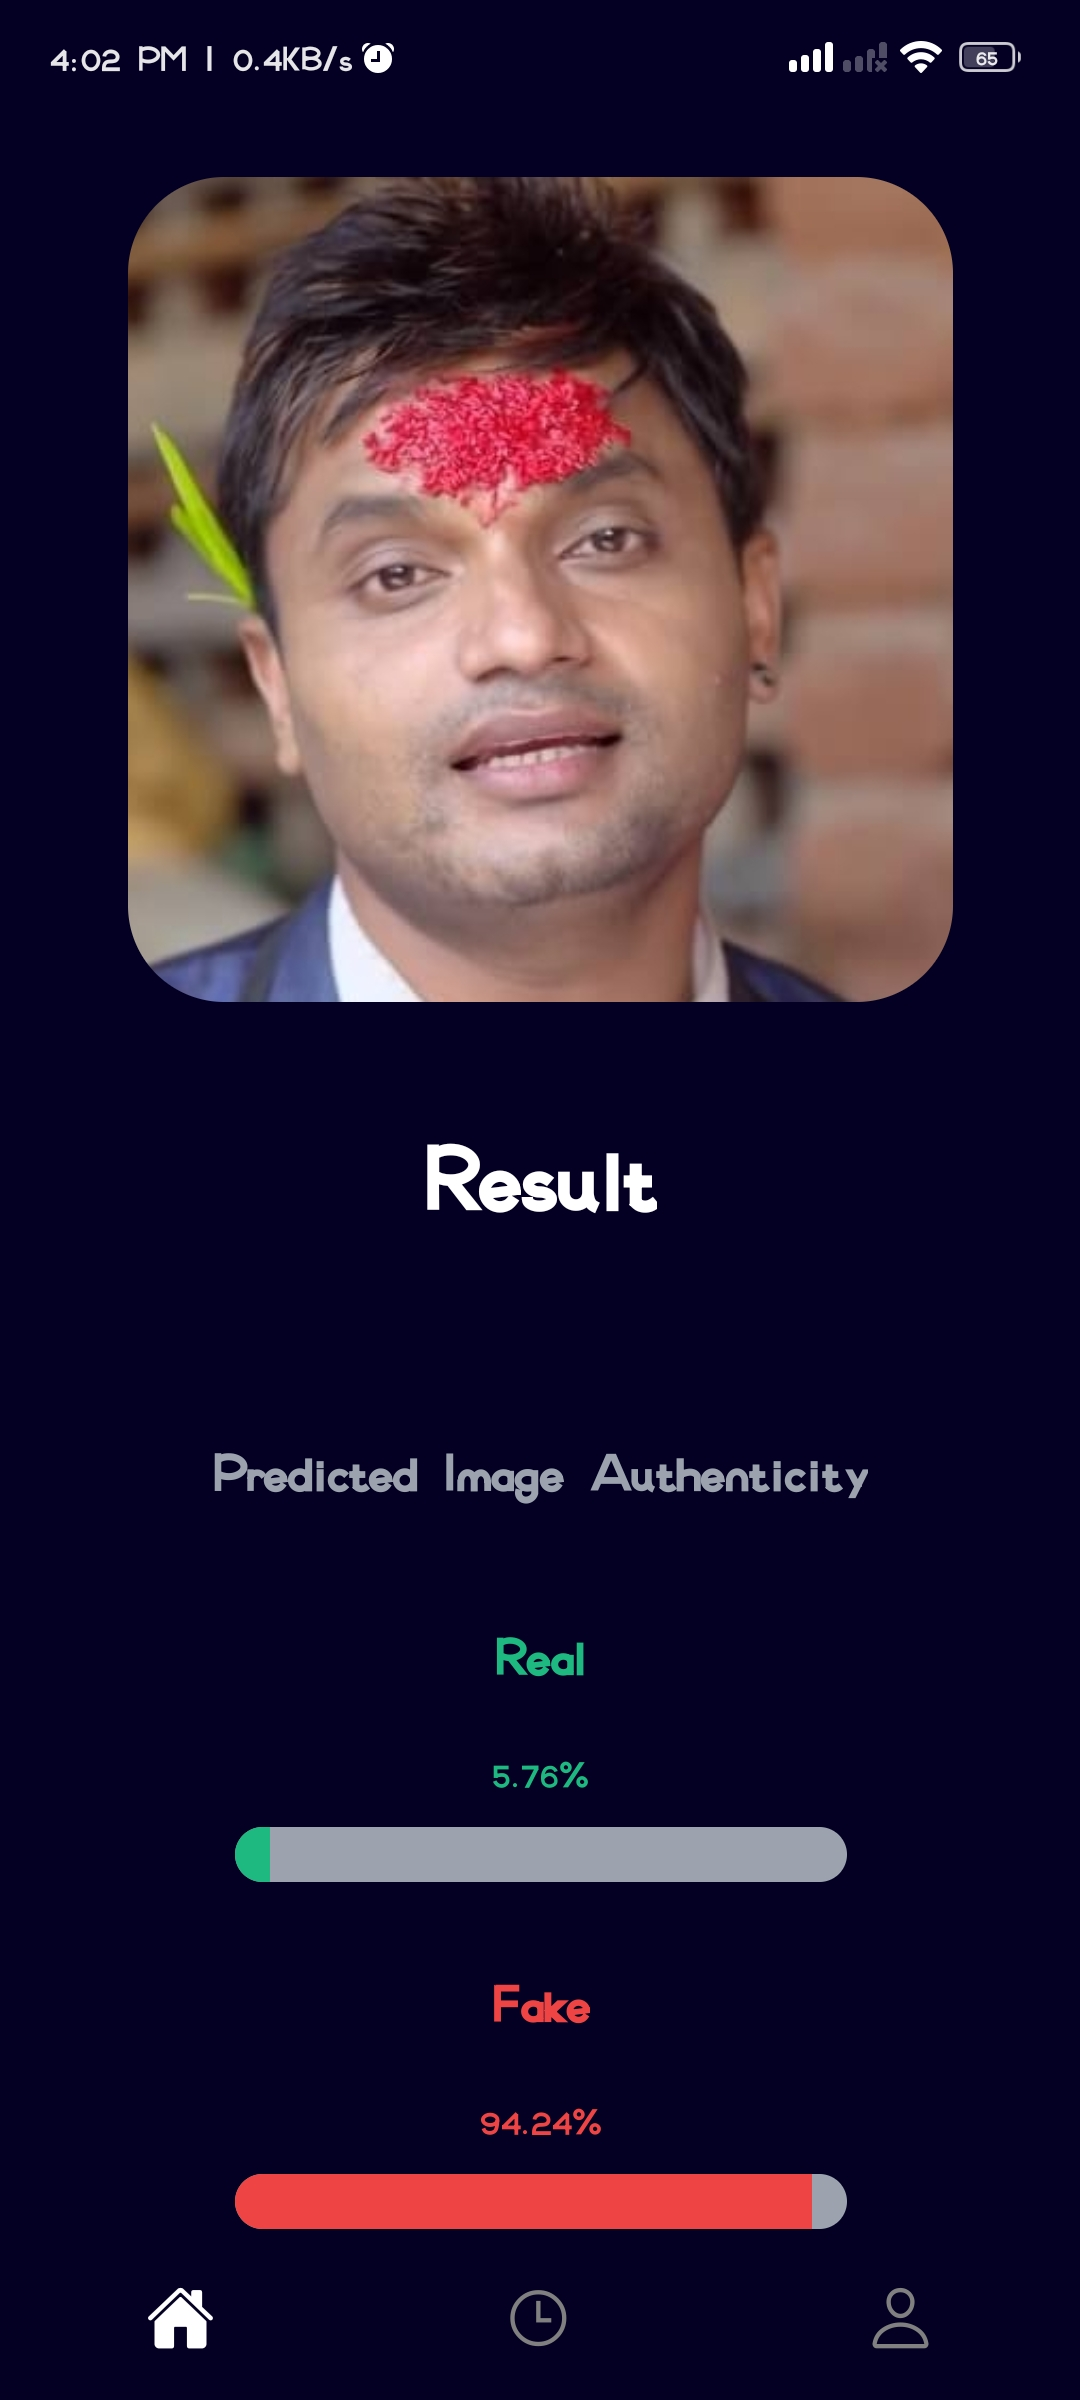
\includegraphics[height =5in ]{img/dashainResult.jpg}
              \caption{\textit{Training Vs Validation loss Curve}}
          \end{figure}


          \newpage

\end{enumerate}
% \subsection{Work Completed}
% \subsubsection{User Interface of Mobile application}
% % \begin{itemize}
% %     \item a
% % \end{itemize}
% \subsubsection{Backend}
% % \begin{itemize}

% % \end{itemize}
% \subsubsection{Machine Learning Model}
% % \begin{itemize}

% % \end{itemize}

% \subsection{Work Remaining}
% % \begin{itemize}

% % \end{itemize}

\newpage
\subsection{UI of Project}
We have used React Native for the development of the mobile application.
Following are the UIs with user authentication, login page and home page where we can upload images to be classified as fake and real.\\

\begin{figure}[ht]
    \centering
    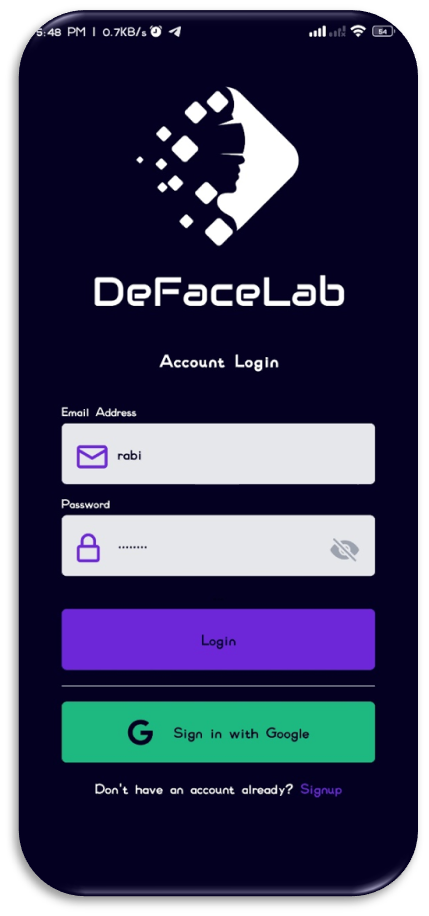
\includegraphics[ height =5in ]{img/loginv3.png}
    \caption{\textit{Login Page }}
\end{figure}

\begin{figure}[ht]
    \centering
    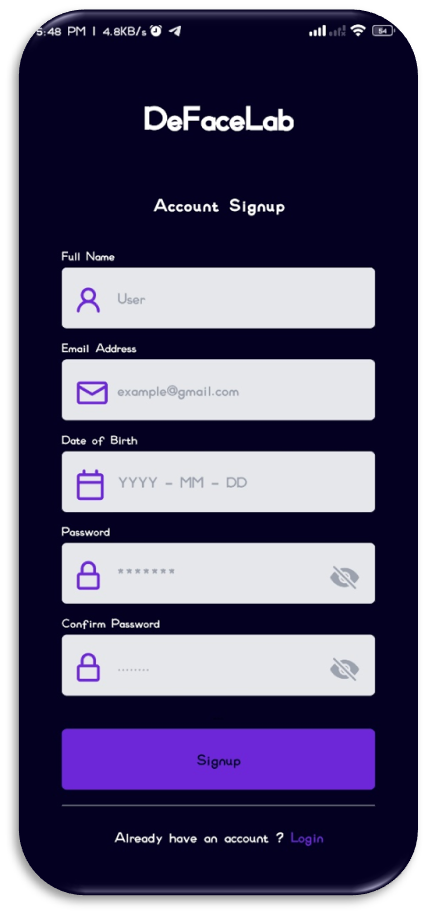
\includegraphics[height= 5in]{img/signup.png}
    \caption{\textit{Sign-up form}}
\end{figure}
\begin{figure}[ht]
    \centering
    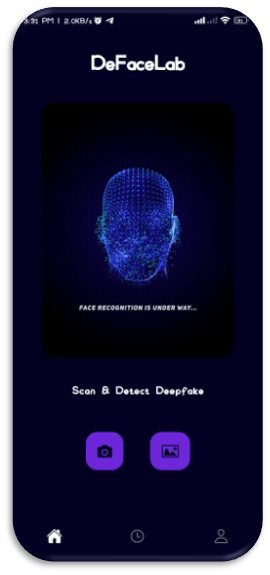
\includegraphics[height =5in ]{img/Homepage.png}
    \caption{\textit{Home Page}}
\end{figure}

\begin{figure}[ht]
    \centering
    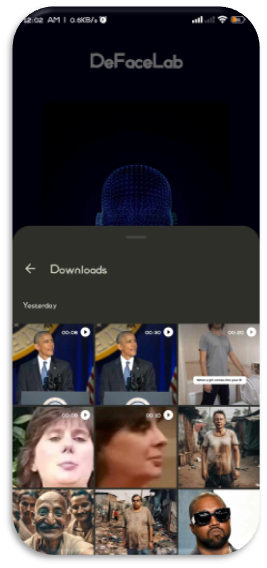
\includegraphics[height =5in ]{img/uploaderv3.png}
    \caption{\textit{Uploader}}
\end{figure}

\begin{figure}[ht]
    \centering
    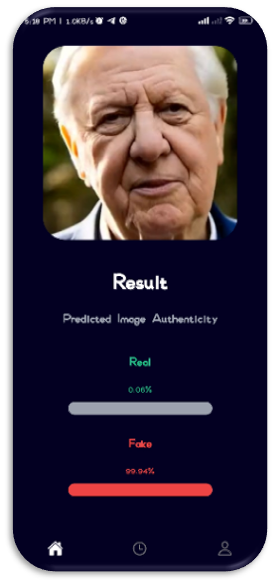
\includegraphics[height= 5in]{img/Results.png}
    \caption{\textit{Result}}
\end{figure}

\begin{figure}[ht]
    \centering
    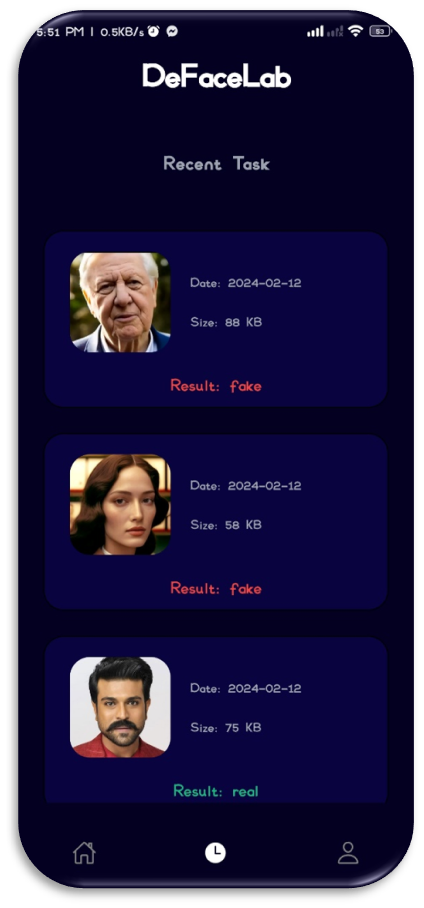
\includegraphics[height= 5in]{img/Historyv2.png}
    \caption{\textit{History page}}
\end{figure}


\begin{figure}[ht]
    \centering
    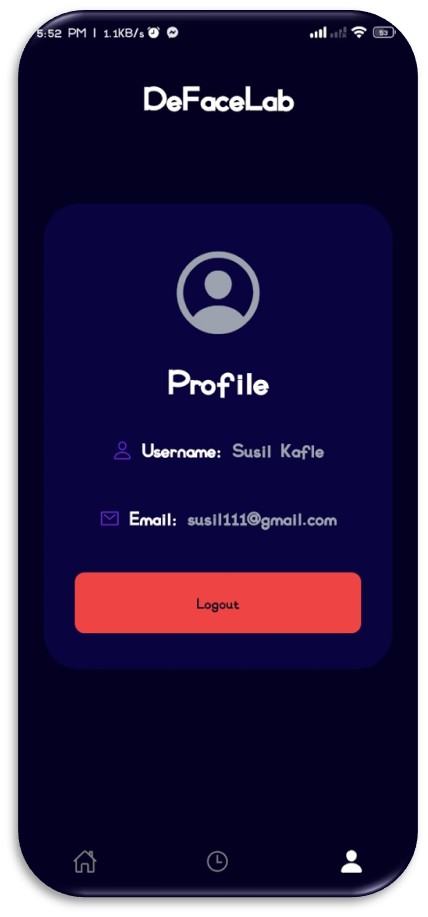
\includegraphics[height= 5in]{img/profilev2.png}
    \caption{\textit{Profile page}}
\end{figure}